\subsection{Numerical Experiments}
Now that we've finally slogged through the presentation of the theory, we can
produce a few numerical experiments. Take, for example, the linear least squares
regression problem with $A \in \mathbb{R}^{n \times m}, x \in \mathbb{R}^m$ and
$b \in \mathbb{R}^n$:
\[
  f(x) = \frac{1}{2}\norm{Ax-b}_2^2 
  = \sum_{k=1}^n 
  \underbrace{ \frac{1}{2} (A_ix - b_i)^2 }_{f_i(x)}
\]
This is a particularily interesting example, as when we examing the stochastic
descent direction of this loss function:
\[
  \nabla f_i(x) = A_{i*}^T(A_{i*}x - b_i), 
  \text{ where }
  A = 
  \begin{bmatrix}
    A_{1*} \\
    \vdots \\
    A_{n*}
  \end{bmatrix}
\]
we notice that the sparsity pattern of $\nabla f_i(x)$ is entirely controlled by
by the sparsity pattern of the rows of $A$. This makes this problem
particularily convinient when trying to understand the effect of sparsity on the
asynchronous noise generated by \hogwild. The original paper \cite{2011NRRW}'s
results required strict assumptions on the sparsity pattern of $\nabla f_i(x)$
in order to guarantee convergence, but as we saw in Theorem
\ref{thm:convexconv}, as long as certain regularity properties are satisfied,
there's no need for such an assumption. Indeed $f$ does satisfy the above,
assuming that $A$ is of full rank%
\footnote{
  One subtle note is that the second condition is actually equivalent to having
  upper bounded maximal eigenvalue. I think we proved this back when we were
  discussing Nesterov's method, and also can be found at this stackexchange
  \url{https://math.stackexchange.com/a/1699082/245618}.
}. Therefore, when $A$ is both sparse and dense, we should see
a $\mathcal{O}(1/k)$ convergence rate, and indeed see figure
\ref{fig:convergence} for the validation of that.
\begin{figure}[!htb]
  \centering
  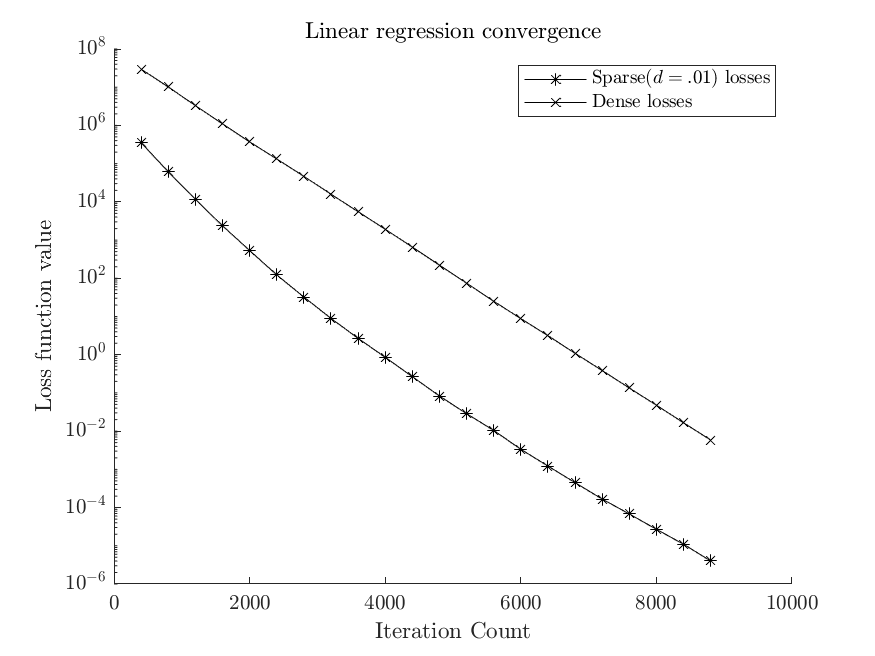
\includegraphics[width=.8\textwidth]{./resources/convergence}
  \caption{
    The matrix Sparse$(d = 0.1)$ is generated by the command {\tt
    sprand(n,m,.01)}. Playing with the density parameter doesn't change the
    shape of the convergence line, but note that denser matrices (since the
    entries are Gaussian) produce a higher initial loss and suffer from more
    asynchronous noise, and therefore require more iterations.
  } \label{fig:convergence}
\end{figure}

\subsubsection{Asynchronous Noise as a Function of Bandedness}
So now that we've seen that, indeed, dense updates enjoy the same convergence
properties as sparser ones, we can also investigate the relationship of
asynchronous noise as a function of sparsity. Since the sampling of the next
data point to be used in a stochastic iterate is done uniformly and
independently, we note that in the interest of minimizing asynchronous noise,
the exact pattern matters less than the number of non-zero elements. Therefore,
an interesting way to represent different sparsity patterns in our linear
regression, is in choosing $A$ banded, and then varying the size of that band.
\begin{definition}
  Let $k \geq 1$ and $A \in \mathbb{R}^{n \times n}$. We denote $A$ as
  a $(k-1)$-banded matrix if $k$ is the maximal integer greater than zero such
  that either the $k$th or the $-k$th diagonal are not-identically zero.
\end{definition}
Now consider the operation of \hogwild\ with two simultaneous threads on the
loss function defined above, with $A$ $k$-banded. Then an lower-bound to the
probability that these two threads do not share an component of $x_i$, which
they need to read/write from/to, is (assuming sampling with replacement) the
probability of picking $i_1, i_2$ uniformly from $[|k+1, \dots, n-k|]$ such that
$[|i_1-k, i_1+k|] \cap [|i_2-k, i_2+k|] = \varnothing$. Via a simple counting
argument, we find that this is:
\[
  \Prob{[|i_1-k, i_1+k|] \cap [|i_2-k, i_2+k|] = \varnothing}
  =
  \frac{\left((n-2k)-(2k+1)\right)_+}{n-2k}
  =
  \frac{\left(n-4k-1\right)_+}{n-2k}
\]
where $(\cdot)_+ = \max(0, \cdot)$. This lower-bound gives us an upperbound on
the probability that they do share a necessary component, one minus the above.
This confirms something we already know, that if $k << n$, then the two threads
are very unlikely to have asynchronous noise. However, with even just $k = n/4$,
then the above probability is zero, and this is just for $P = 2$. I had wanted
to calculate the $k$ taking the above to zero as a function of $P$, but the
analysis quickly becomes intractible for $P \geq 3$, barring a nice counting
argument I don't see. Regardless, as long as we can measure asynchronous noise,
we can get an idea of how it increases as a function of $k$.

To construct an experiment to see this, let $x_k$ ($k$ not a component, but an
parameter) be the final iterate of \hogwild, as applied to the linear regression
problem with $A$ $k$-banded. Then supposing we hold some solution $x^*$ constant
among all $k$, then we can view $f(x_k)$ as a random-variable, whose variance
characterizes the amount of asynchronous noise experienced throughout
computation, as the sequential algorithm (assuming the random choice of
stochastic data points is seeded between intervals) will have $\Var{f(x_k)} = 0,
\forall k$. See figure \ref{fig:variances} for the results of such an
experiment.
\begin{figure}[!htb]
  \centering
  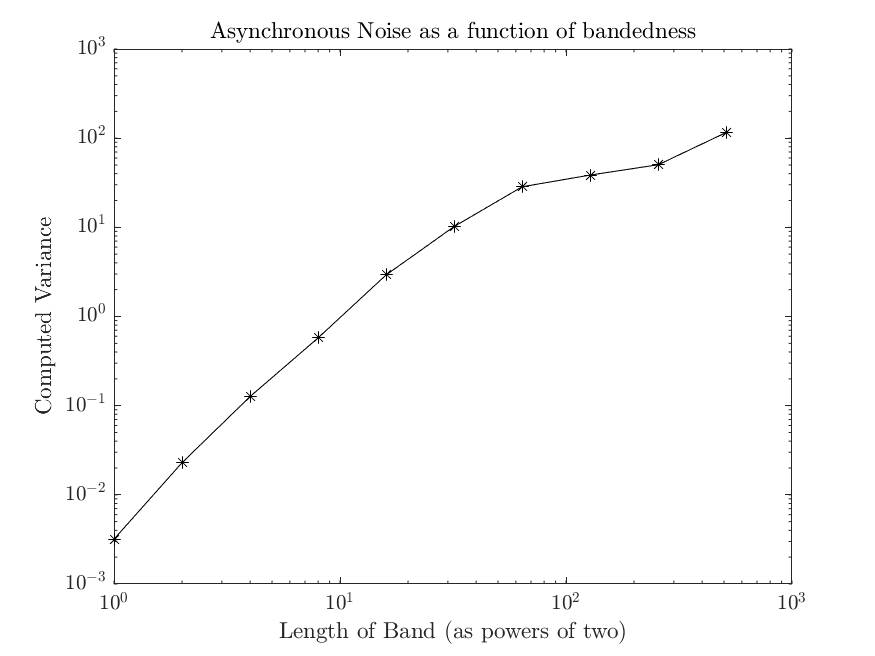
\includegraphics[width=.8\textwidth]{./resources/banded_asyncnoise}
  \caption{
  } \label{fig:variances}
\end{figure}
